% Options for packages loaded elsewhere
\PassOptionsToPackage{unicode}{hyperref}
\PassOptionsToPackage{hyphens}{url}
%
\documentclass[
]{article}
\usepackage{amsmath,amssymb}
\usepackage{iftex}
\ifPDFTeX
  \usepackage[T1]{fontenc}
  \usepackage[utf8]{inputenc}
  \usepackage{textcomp} % provide euro and other symbols
\else % if luatex or xetex
  \usepackage{unicode-math} % this also loads fontspec
  \defaultfontfeatures{Scale=MatchLowercase}
  \defaultfontfeatures[\rmfamily]{Ligatures=TeX,Scale=1}
\fi
\usepackage{lmodern}
\ifPDFTeX\else
  % xetex/luatex font selection
\fi
% Use upquote if available, for straight quotes in verbatim environments
\IfFileExists{upquote.sty}{\usepackage{upquote}}{}
\IfFileExists{microtype.sty}{% use microtype if available
  \usepackage[]{microtype}
  \UseMicrotypeSet[protrusion]{basicmath} % disable protrusion for tt fonts
}{}
\makeatletter
\@ifundefined{KOMAClassName}{% if non-KOMA class
  \IfFileExists{parskip.sty}{%
    \usepackage{parskip}
  }{% else
    \setlength{\parindent}{0pt}
    \setlength{\parskip}{6pt plus 2pt minus 1pt}}
}{% if KOMA class
  \KOMAoptions{parskip=half}}
\makeatother
\usepackage{xcolor}
\usepackage[margin=1in]{geometry}
\usepackage{color}
\usepackage{fancyvrb}
\newcommand{\VerbBar}{|}
\newcommand{\VERB}{\Verb[commandchars=\\\{\}]}
\DefineVerbatimEnvironment{Highlighting}{Verbatim}{commandchars=\\\{\}}
% Add ',fontsize=\small' for more characters per line
\usepackage{framed}
\definecolor{shadecolor}{RGB}{248,248,248}
\newenvironment{Shaded}{\begin{snugshade}}{\end{snugshade}}
\newcommand{\AlertTok}[1]{\textcolor[rgb]{0.94,0.16,0.16}{#1}}
\newcommand{\AnnotationTok}[1]{\textcolor[rgb]{0.56,0.35,0.01}{\textbf{\textit{#1}}}}
\newcommand{\AttributeTok}[1]{\textcolor[rgb]{0.13,0.29,0.53}{#1}}
\newcommand{\BaseNTok}[1]{\textcolor[rgb]{0.00,0.00,0.81}{#1}}
\newcommand{\BuiltInTok}[1]{#1}
\newcommand{\CharTok}[1]{\textcolor[rgb]{0.31,0.60,0.02}{#1}}
\newcommand{\CommentTok}[1]{\textcolor[rgb]{0.56,0.35,0.01}{\textit{#1}}}
\newcommand{\CommentVarTok}[1]{\textcolor[rgb]{0.56,0.35,0.01}{\textbf{\textit{#1}}}}
\newcommand{\ConstantTok}[1]{\textcolor[rgb]{0.56,0.35,0.01}{#1}}
\newcommand{\ControlFlowTok}[1]{\textcolor[rgb]{0.13,0.29,0.53}{\textbf{#1}}}
\newcommand{\DataTypeTok}[1]{\textcolor[rgb]{0.13,0.29,0.53}{#1}}
\newcommand{\DecValTok}[1]{\textcolor[rgb]{0.00,0.00,0.81}{#1}}
\newcommand{\DocumentationTok}[1]{\textcolor[rgb]{0.56,0.35,0.01}{\textbf{\textit{#1}}}}
\newcommand{\ErrorTok}[1]{\textcolor[rgb]{0.64,0.00,0.00}{\textbf{#1}}}
\newcommand{\ExtensionTok}[1]{#1}
\newcommand{\FloatTok}[1]{\textcolor[rgb]{0.00,0.00,0.81}{#1}}
\newcommand{\FunctionTok}[1]{\textcolor[rgb]{0.13,0.29,0.53}{\textbf{#1}}}
\newcommand{\ImportTok}[1]{#1}
\newcommand{\InformationTok}[1]{\textcolor[rgb]{0.56,0.35,0.01}{\textbf{\textit{#1}}}}
\newcommand{\KeywordTok}[1]{\textcolor[rgb]{0.13,0.29,0.53}{\textbf{#1}}}
\newcommand{\NormalTok}[1]{#1}
\newcommand{\OperatorTok}[1]{\textcolor[rgb]{0.81,0.36,0.00}{\textbf{#1}}}
\newcommand{\OtherTok}[1]{\textcolor[rgb]{0.56,0.35,0.01}{#1}}
\newcommand{\PreprocessorTok}[1]{\textcolor[rgb]{0.56,0.35,0.01}{\textit{#1}}}
\newcommand{\RegionMarkerTok}[1]{#1}
\newcommand{\SpecialCharTok}[1]{\textcolor[rgb]{0.81,0.36,0.00}{\textbf{#1}}}
\newcommand{\SpecialStringTok}[1]{\textcolor[rgb]{0.31,0.60,0.02}{#1}}
\newcommand{\StringTok}[1]{\textcolor[rgb]{0.31,0.60,0.02}{#1}}
\newcommand{\VariableTok}[1]{\textcolor[rgb]{0.00,0.00,0.00}{#1}}
\newcommand{\VerbatimStringTok}[1]{\textcolor[rgb]{0.31,0.60,0.02}{#1}}
\newcommand{\WarningTok}[1]{\textcolor[rgb]{0.56,0.35,0.01}{\textbf{\textit{#1}}}}
\usepackage{graphicx}
\makeatletter
\def\maxwidth{\ifdim\Gin@nat@width>\linewidth\linewidth\else\Gin@nat@width\fi}
\def\maxheight{\ifdim\Gin@nat@height>\textheight\textheight\else\Gin@nat@height\fi}
\makeatother
% Scale images if necessary, so that they will not overflow the page
% margins by default, and it is still possible to overwrite the defaults
% using explicit options in \includegraphics[width, height, ...]{}
\setkeys{Gin}{width=\maxwidth,height=\maxheight,keepaspectratio}
% Set default figure placement to htbp
\makeatletter
\def\fps@figure{htbp}
\makeatother
\setlength{\emergencystretch}{3em} % prevent overfull lines
\providecommand{\tightlist}{%
  \setlength{\itemsep}{0pt}\setlength{\parskip}{0pt}}
\setcounter{secnumdepth}{-\maxdimen} % remove section numbering
\ifLuaTeX
  \usepackage{selnolig}  % disable illegal ligatures
\fi
\usepackage{bookmark}
\IfFileExists{xurl.sty}{\usepackage{xurl}}{} % add URL line breaks if available
\urlstyle{same}
\hypersetup{
  pdftitle={Wine Dataset Clustering Analysis},
  hidelinks,
  pdfcreator={LaTeX via pandoc}}

\title{Wine Dataset Clustering Analysis}
\author{}
\date{\vspace{-2.5em}}

\begin{document}
\maketitle

\subsection{Load Dataset}\label{load-dataset}

The necessary libraries and the wine dataset are loaded.

\begin{Shaded}
\begin{Highlighting}[]
\FunctionTok{library}\NormalTok{(tidyverse)}
\end{Highlighting}
\end{Shaded}

\begin{verbatim}
## -- Attaching core tidyverse packages ------------------------ tidyverse 2.0.0 --
## v dplyr     1.1.4     v readr     2.1.5
## v forcats   1.0.0     v stringr   1.5.1
## v ggplot2   3.5.1     v tibble    3.2.1
## v lubridate 1.9.3     v tidyr     1.3.1
## v purrr     1.0.2     
## -- Conflicts ------------------------------------------ tidyverse_conflicts() --
## x dplyr::filter() masks stats::filter()
## x dplyr::lag()    masks stats::lag()
## i Use the conflicted package (<http://conflicted.r-lib.org/>) to force all conflicts to become errors
\end{verbatim}

\begin{Shaded}
\begin{Highlighting}[]
\NormalTok{data\_url }\OtherTok{\textless{}{-}} \StringTok{\textquotesingle{}https://raw.githubusercontent.com/koimabrian/Datasets/refs/heads/main/Wine.csv\textquotesingle{}}
\NormalTok{Wine }\OtherTok{\textless{}{-}} \FunctionTok{read.csv}\NormalTok{(data\_url, }\AttributeTok{comment =} \StringTok{"\#"}\NormalTok{)  }\CommentTok{\# Handle potential comments in the CSV}
\FunctionTok{head}\NormalTok{(Wine)}
\end{Highlighting}
\end{Shaded}

\begin{verbatim}
##   Obs   Rating    Price   Alcohol Residual_Sugar  Sulphates       pH Country
## 1   1 66.09628 42.35785 12.884478       1.723964 1.82236164 3.094826   Italy
## 2   2 26.29778 18.07262 10.788513       2.717204 1.25833852 3.687788  Canada
## 3   3 57.55450 27.33195  9.836948       1.412335 0.02351161 3.463087  Canada
## 4   4 46.55640 22.75134 12.022274       3.068457 1.79914031 1.544849   Italy
## 5   5 49.40503 14.39930 11.442785       2.994345 1.06218391 3.032852  France
## 6   6 41.32942 18.01701 11.667942       1.631718 0.85062170 2.191800  Canada
\end{verbatim}

\subsection{Standardize Continuous
Variables}\label{standardize-continuous-variables}

The continuous variables (excluding observation number and country) are
scaled.

\begin{Shaded}
\begin{Highlighting}[]
\NormalTok{data }\OtherTok{\textless{}{-}}\NormalTok{ Wine }\SpecialCharTok{\%\textgreater{}\%} \FunctionTok{select}\NormalTok{(}\SpecialCharTok{{-}}\NormalTok{Obs, }\SpecialCharTok{{-}}\NormalTok{Country) }\SpecialCharTok{\%\textgreater{}\%} \FunctionTok{scale}\NormalTok{()}
\end{Highlighting}
\end{Shaded}

\subsection{Create Clusters with
K-Means}\label{create-clusters-with-k-means}

The k-means algorithm is applied to the standardized data, setting the
number of clusters to 3.

\begin{Shaded}
\begin{Highlighting}[]
\NormalTok{kmeans\_result }\OtherTok{\textless{}{-}} \FunctionTok{kmeans}\NormalTok{(data, }\AttributeTok{centers =} \DecValTok{3}\NormalTok{, }\AttributeTok{iter.max =} \DecValTok{100}\NormalTok{, }\AttributeTok{nstart =} \DecValTok{100}\NormalTok{)}
\NormalTok{kmeans\_result}
\end{Highlighting}
\end{Shaded}

\begin{verbatim}
## K-means clustering with 3 clusters of sizes 43, 25, 32
## 
## Cluster means:
##          Rating       Price    Alcohol Residual_Sugar  Sulphates          pH
## 1 -0.7611830170 -0.74488647 -0.3311789    -0.48277078 -0.1169446  0.37747968
## 2  0.0005649203 -0.09531108  0.7695537     0.73705964  0.7738343 -0.71133001
## 3  1.0223983350  1.07540297 -0.1561923     0.07289539 -0.4474138  0.04848825
## 
## Clustering vector:
##   [1] 3 1 1 2 1 1 2 2 3 3 1 1 1 1 1 3 3 1 1 1 2 2 3 3 1 1 3 2 1 3 1 3 3 2 3 1 3
##  [38] 2 3 1 1 1 3 1 2 3 1 1 3 3 2 2 1 3 1 1 3 2 1 1 2 1 3 2 3 3 3 2 1 1 1 1 1 2
##  [75] 3 1 1 2 2 1 1 3 2 2 1 3 1 2 2 2 3 1 2 3 3 3 3 1 2 1
## 
## Within cluster sum of squares by cluster:
## [1] 156.1271 114.3882 119.1354
##  (between_SS / total_SS =  34.4 %)
## 
## Available components:
## 
## [1] "cluster"      "centers"      "totss"        "withinss"     "tot.withinss"
## [6] "betweenss"    "size"         "iter"         "ifault"
\end{verbatim}

\subsection{Determine the Optimal Number of
Clusters}\label{determine-the-optimal-number-of-clusters}

To identify the optimal number of clusters, the within-cluster sum of
squares (WSS), silhouette method, and gap statistic are visualized.

\begin{Shaded}
\begin{Highlighting}[]
\FunctionTok{library}\NormalTok{(factoextra)}
\CommentTok{\# WSS plot}
\FunctionTok{fviz\_nbclust}\NormalTok{(data, kmeans, }\AttributeTok{method =} \StringTok{"wss"}\NormalTok{)}
\end{Highlighting}
\end{Shaded}

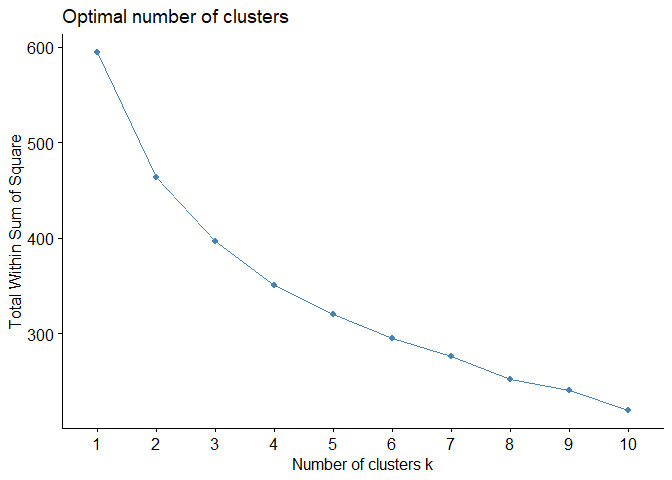
\includegraphics{README_files/figure-latex/optimal-cluster-number-1.pdf}

\begin{Shaded}
\begin{Highlighting}[]
\CommentTok{\# Silhouette plot}
\FunctionTok{fviz\_nbclust}\NormalTok{(data, kmeans, }\AttributeTok{method =} \StringTok{"silhouette"}\NormalTok{)}
\end{Highlighting}
\end{Shaded}

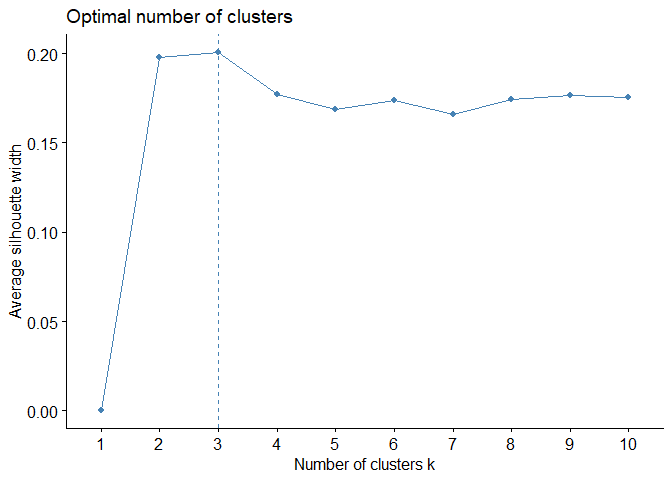
\includegraphics{README_files/figure-latex/optimal-cluster-number-2.pdf}

\begin{Shaded}
\begin{Highlighting}[]
\CommentTok{\# Gap statistic}
\FunctionTok{fviz\_nbclust}\NormalTok{(data, kmeans, }\AttributeTok{method =} \StringTok{"gap\_stat"}\NormalTok{)}
\end{Highlighting}
\end{Shaded}

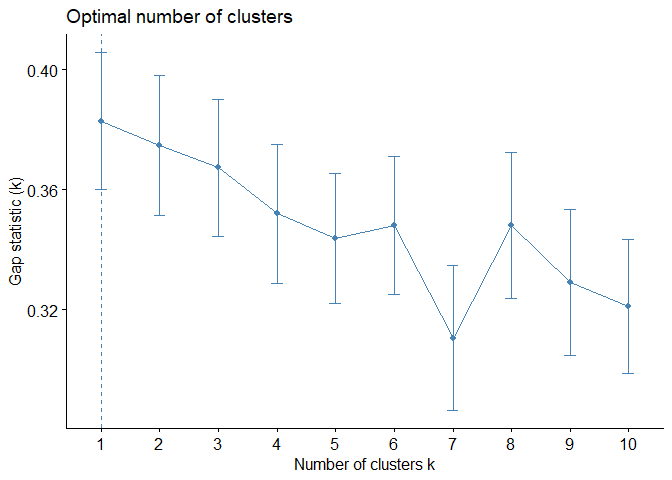
\includegraphics{README_files/figure-latex/optimal-cluster-number-3.pdf}

\subsection{Cluster Visualization}\label{cluster-visualization}

Clusters are visualized in a biplot, and then plotted using the original
variables (Rating vs Price).

\begin{Shaded}
\begin{Highlighting}[]
\CommentTok{\# Cluster biplot}
\FunctionTok{fviz\_cluster}\NormalTok{(}\FunctionTok{kmeans}\NormalTok{(data, }\AttributeTok{centers =} \DecValTok{3}\NormalTok{, }\AttributeTok{iter.max =} \DecValTok{100}\NormalTok{, }\AttributeTok{nstart =} \DecValTok{100}\NormalTok{), }\AttributeTok{data =}\NormalTok{ data)}
\end{Highlighting}
\end{Shaded}

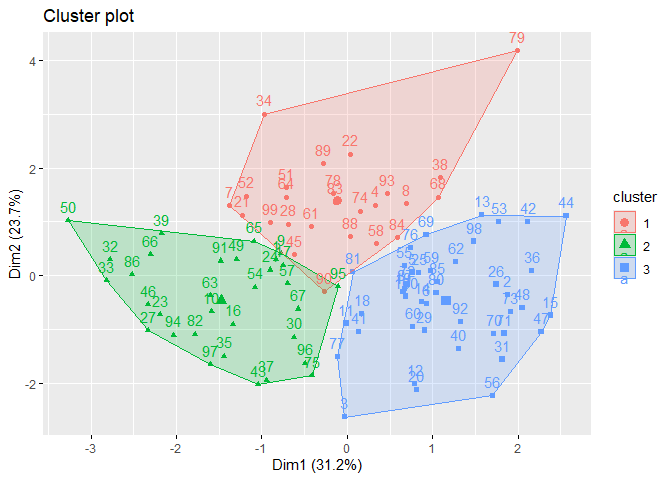
\includegraphics{README_files/figure-latex/cluster-biplot-1.pdf}

\subsubsection{Clusters with Original
Variables}\label{clusters-with-original-variables}

Cluster labels are added to the original dataset, and clusters are
visualized using the Rating and Price variables.

\begin{Shaded}
\begin{Highlighting}[]
\NormalTok{clusters }\OtherTok{\textless{}{-}} \FunctionTok{kmeans}\NormalTok{(data, }\AttributeTok{centers =} \DecValTok{3}\NormalTok{, }\AttributeTok{iter.max =} \DecValTok{100}\NormalTok{, }\AttributeTok{nstart =} \DecValTok{100}\NormalTok{)}
\NormalTok{Wine }\OtherTok{\textless{}{-}}\NormalTok{ Wine }\SpecialCharTok{|\textgreater{}} \FunctionTok{mutate}\NormalTok{(}\AttributeTok{cluster =}\NormalTok{ clusters}\SpecialCharTok{$}\NormalTok{cluster)}

\CommentTok{\# Plot clusters using Rating and Price}
\NormalTok{Wine }\SpecialCharTok{|\textgreater{}} \FunctionTok{ggplot}\NormalTok{(}\FunctionTok{aes}\NormalTok{(}\AttributeTok{x =}\NormalTok{ Rating, }\AttributeTok{y =}\NormalTok{ Price, }\AttributeTok{col =} \FunctionTok{as.factor}\NormalTok{(cluster))) }\SpecialCharTok{+} 
  \FunctionTok{geom\_point}\NormalTok{() }\SpecialCharTok{+} 
  \FunctionTok{labs}\NormalTok{(}\AttributeTok{title =} \StringTok{"Wine Clusters by Rating and Price"}\NormalTok{, }\AttributeTok{color =} \StringTok{"Cluster"}\NormalTok{)}
\end{Highlighting}
\end{Shaded}

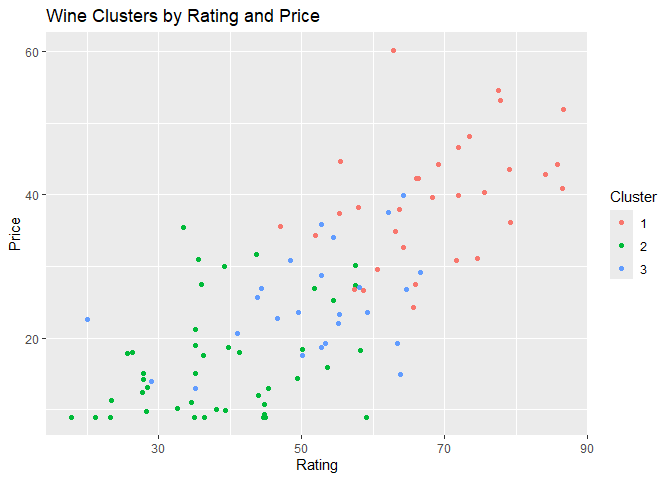
\includegraphics{README_files/figure-latex/original-variable-clusters-1.pdf}

\end{document}
